\documentclass[12pt]{article}

\usepackage[parfill]{parskip}

\usepackage[utf8]{inputenc}

% A package for setting layout and margins for your thesis 
\usepackage[a4paper]{geometry}

\usepackage[english, estonian]{babel}

% General packages for math in general, theorems and symbols 
% Read ftp://ftp.ams.org/ams/doc/amsmath/short-math-guide.pdf for further information
\usepackage{amsmath} 
\usepackage{amsthm}
\usepackage{amssymb}

% Packages for building tables and tabulars 
\usepackage{array}
\usepackage{tabu}   % Wide lines in tables
\usepackage{xspace} % Non-eatable spaces in macros

% Including graphical images and setting the figure directory
\usepackage{graphicx}
\graphicspath{{figures/}}

% Packages for getting clickable links in PDF file
\usepackage{hyperref}
\usepackage[all]{hypcap}

% Packages for defining colourful text together with some colours
\usepackage{color}
\usepackage{xcolor} 
%\definecolor{dkgreen}{rgb}{0,0.6,0}
%\definecolor{gray}{rgb}{0.5,0.5,0.5}
\definecolor{mauve}{rgb}{0.58,0,0.82}

% Standard package for drawing algorithms
% Since the thesis in article format we must define \chapter for
% the package algorithm2e (otherwise obscure errors occur) 
\let\chapter\section
\usepackage[ruled, vlined, linesnumbered]{algorithm2e}

% Fix a  set of keywords which you use inside algorithms
\SetKw{True}{true}
\SetKw{False}{false}
\SetKwData{typeInt}{Int}
\SetKwData{typeRat}{Rat}
\SetKwData{Defined}{Defined}
\SetKwFunction{parseStatement}{parseStatement}

% Nice todo notes
\usepackage{todonotes}

% Proper way to create coloured code listings
\usepackage{listings}
\lstset{ 
  %language=python,                % the language of the code
  language=C++,
  basicstyle=\footnotesize,        % the size of the fonts that are used for the code
  %numbers=left,                   % where to put the line-numbers
  %numberstyle=\footnotesize,      % the size of the fonts that are used for the line-numbers
  numberstyle=\tiny\color{gray}, 
  stepnumber=1,                    % the step between two line-numbers. If it's 1, each line 
                                   % will be numbered
  numbersep=5pt,                   % how far the line-numbers are from the code
  backgroundcolor=\color{white},   % choose the background color. You must add \usepackage{color}
  showspaces=false,                % show spaces adding particular underscores
  showstringspaces=false,          % underline spaces within strings
  showtabs=false,                  % show tabs within strings adding particular underscores
  frame = lines,
  %frame=single,                   % adds a frame around the code
  rulecolor=\color{black},		   % if not set, the frame-color may be changed on line-breaks within 
                                   % not-black text (e.g. commens (green here))
  tabsize=2,                       % sets default tabsize to 2 spaces
  captionpos=b,                    % sets the caption-position to bottom
  breaklines=true,                 % sets automatic line breaking
  breakatwhitespace=false,         % sets if automatic breaks should only happen at whitespace
  %title=\lstname,                 % show the filename of files included with \lstinputlisting;
                                   % also try caption instead of title
                                   % also try caption instead of title
  keywordstyle=\color{blue},       % keyword style
  commentstyle=\color{dkgreen},    % comment style
  stringstyle=\color{mauve},       % string literal style
  escapeinside={\%*}{*)},          % if you want to add a comment within your code
  morekeywords={*,game, fun}       % if you want to add more keywords to the set
}


% Obscure packages to write logic formulae and program semantics
% Unless you do a bachelor thesis on program semantics or static code analysis you do not need that
% http://logicmatters.net/resources/ndexamples/proofsty3.html <= writing type rules => use semantic::inference
% ftp://tug.ctan.org/tex-archive/macros/latex/contrib/semantic/semantic.pdf
\usepackage{proof}
\usepackage{semantic} 
\setlength{\inferLineSkip}{4pt}
\def\predicatebegin #1\predicateend{$\Gamma \vdash #1$}

% If you really want to draw figures in LaTeX use packages tikz or pstricks
% However, getting a corresponding illustrations is really painful  

% Define your favorite macros that you use inside the thesis 
% Name followed by non-removable space
\newcommand{\proveit}{ProveIt\xspace}

% Macros that make sure that the math mode is set
\newcommand{\typeF}[1] {\ensuremath{\mathsf{type_{#1}}}\xspace}
\newcommand{\opDiv}{\ensuremath{\backslash \mathsf{div}}\xspace} 

% Nice Todo box
\newcommand{\TODO}{\todo[inline]}

% A way to define theorems and lemmata
\newtheorem{theorem}{Theorem}


%%% BEGIN DOCUMENT
\begin{document}

% BEGIN TITLE PAGE
\thispagestyle{empty}
\begin{center}

\large
UNIVERSITY OF TARTU\\[2mm]
Institute of Computer Science\\
Computer Science Curriculum\\[2mm]

%\vspace*{\stretch{5}}
\vspace{25mm}

\Large Sten Sootla

\vspace{4mm}

\huge Analysing information distribution in complex systems

%\vspace*{\stretch{7}}
\vspace{20mm}

\Large Bachelor's Thesis (9 ECTS)

\end{center}

\vspace{2mm}

\begin{flushright}
 {
 \setlength{\extrarowheight}{5pt}
 \begin{tabular}{r l} 
  \sffamily Supervisor: & \sffamily Raul Vicente Zafra, PhD \\
  \sffamily Supervisor: & \sffamily Dirk Oliver Theis, PhD
 \end{tabular}
 }
\end{flushright}

%\vspace*{\stretch{3}}
\vspace{10mm}

%{\noindent Author: .................................................................................... ``.....'' ..........\hskip16pt 2048}
\vspace{2mm}


%{\noindent Supervisor: ............................................................................... ``.....'' ..........\hskip16pt 2048}

\vspace{2mm}

%{\noindent Supervisor: ............................................................................... ``.....'' ..........\hskip16pt 2048}

\vspace{8mm}


\vfill
\centerline{Tartu 2017}

% END TITLE PAGE

\selectlanguage{english}

\newpage
\tableofcontents

\newpage
\section{Introduction}

\selectlanguage{estonian}

\textcolor{red}{Vabandust, et sissejuhatust veel hetkel ei ole. Minu jaoks on alati sissejuhatus kõige raskem osa olnud kirjatükkides, ja pole olnud kordagi, kus sissejuhatus poleks jäänud absoluutselt viimaseks osaks. Sissejuhatus annab ülevaate kogu minu tööle, mistõttu arvan, et seda on paslik koostada siis, kui on millest ülevaade teha.}

\textcolor{red}{Lubage mul tuua näide elust. Kaks aastat tagasi kohtusin tüdrukuga, kes on nüüdseks minu ekstüdruk. Kui minult oleks palutud kirjutada sel hetkel ülevaade oma ülejäänud elust, siis suure osa kirjaruumist oleks kahtlemata hõlmanud see tüdruk. Õnneks ei alustanud ma tol hetkel ülevaate andmist oma tulevikust, sest nüüd oleme juba kuid lahus. Mõistagi muudab see resultaat minu elulooraamatu sisu märgatavalt. Hea, et ei hakanud elulooraamatusse ennatlikult tulevikust kirjutama, muidu oleks see olnud mahavisatud aeg. Veelgi enam, õnnelikel aegadel kirjutatud tulevikuplaanide lugemine ei oleks hetkel kindlasti kõige tervislikum ajaviide, mil suhe juba purunenud.}

\textcolor{red}{Kui sissejuhatuse eesmärk nii varajases staadiumis on lihtsalt töö läbimõtlemine ja kirjutamisoskuse demonstreerimine, siis ehk piisab hetkel sisukorrast ja esimesest peatükist, mis tasapisi edeneb. Kui mitte, siis mõistagi tuleb mul see sissejuhatus lihtsalt ära teha kiiremas korras :/}

\selectlanguage{english}

In Chapter 1, the basics of classical information theory and partial information decomposition are covered. The chapter ends with an overview of the numerical estimator for PID.

The subsequent 3 chapters each introduce a specific complex system and the results of measuring information distribution in it. 

Chapter 2 - Elementary Cellular Automata 
Chapter 3 - Ising model 
Chapter 4 - Artificial Neural Networks

In the final, concluding chapter, a summary of the contributions of this thesis is given, alongside suggestions for further work. 

\newpage
\section{Background}

\subsection{Classical information theory}

In order to understand partial information decomposition, which is the mathematical framework that is used in this thesis to analyse complex systems, a solid understanding of basic information theory is essential. This subsection fills that gap, giving a brief overview of the fundamental concepts of information theory. Where appropriate, the rather abstract definitions are further elaborated on by providing the reader with intuitive explanations and concrete examples.

In the following discussion, when not specified otherwise, it is assumed that $X$ is a discrete random variable with possible realizations from the set $\{x_1, x_2, ..., x_n\}$ and a probability mass function $p_X(x_i) = Pr\{X = x_i\} \ (i = 1, ..., n)$. Similiarly, $Y$ is a discrete random variable with possible realizations from the set $\{y_1, y_2, ..., y_m\}$ and a probability mass function $p_Y(y_j) = Pr\{Y = y_j\} \ (j = 1, ..., m)$.

\subsubsection{Entropy}

The most fundamental quantitiy of information theory is \textit{entropy}, being a basic building block of all the other information theoretic functionals introduced in this thesis. The entropy of the random variable $X$ is defined by Shannon \cite{shannon} as follows: 

\begin{equation}
H(X) = -\sum_{i=1}^{n} p_X(x_i) \log_2 p(x_i)
\label{eq:entropy}
\end{equation}

If the base of the logarithm is 2, the units the entropy is measured in are called \textit{bits}. Another common base for the logarithm is Euler's number $e \approx 2.718$, in which case the units of measurment are called \textit{nats}.

Intuitively, entropy can be thought of as the average amount of uncertainty of a random variable. It is indeed an \textit{average}, as the uncertainty of a single relatization of $x_i$ of a random variable $X$ can be quantified by $-log_2 p(x_i)$. Viewed from this angle, the definition of entropy can be rewritten as an expectation of the random variable $-\log_2 p(X)$: 

$$H(X) = \mathbb{E} \left[ - \log_2 p(X) \right] = \mathbb{E} \left[ \log_2 \frac{1}{p(X)} \right].$$

To see why this intuition should correspond to the mathematical definition, it is instructive to look at a concrete example, inspired by \cite{cover-thomas}. Suppose we have a binary random variable $X$, defined as follows: 

$$X = \begin{cases} 1 & \mbox{with probability } p, \\ 0, & \mbox{with probability } 1-p. \end{cases}$$

Essentially, this random variable encodes a coin toss, where the probability of flipping heads is $p$ and the probability of flipping tails is $1-p$. If $p=0.5$, the coin is considered to be unbiased, otherwise it is called biased.

Using equation \ref{eq:entropy}, it is straightforward to calculate the entropy of $X$, given some specific value of $p$. Figure \ref{fig:entropy} graphs the value of $H(X)$ against every possible $p \in \left[ 0, 1 \right]$. When $p \in \{0, 1\}$, then the outcome of the coin toss is completely deterministic, meaning there is no uncertainty in the outcome. Accordingly, the entropy is 0 at these points. Conversely, when the coin is fair, we are completely uncertain about the outcome, unable to favour neither heads or tails. Again, the mathematical definition and intuition agree, as the entropy is indeed at its maximum when $p = 0.5$.

\begin{figure} [h]
\begin{center}
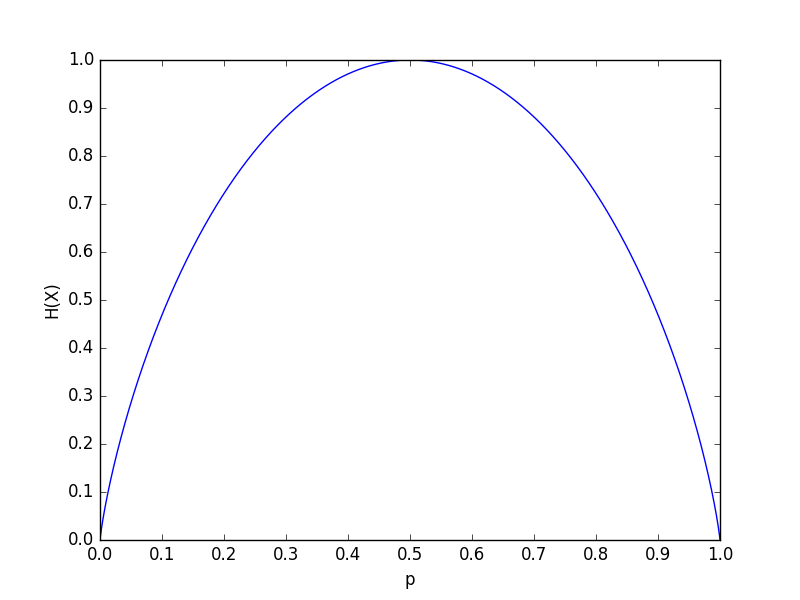
\includegraphics[width=0.8\textwidth]{entropy}
\caption{Entropy of $X$ plotted against the value of $p$.}
\label{fig:entropy}
\end{center}
\end{figure}

\subsubsection{Joint and Conditional Entropy}

Let the joint distribution of the random variables $X$ and $Y$ be $p(x_i, y_j) = Pr\{X = x_i, Y = y_j\} \ (i = 1, ..., n; \ j = 1, ..., m)$. The \textit{joint entropy} \cite{cover-thomas} of the pair $(X,Y)$ is defined as 

\begin{equation}
H(X,Y) = -\sum_{i=1}^n \sum_{j=1}^m p(x_i,y_j) \log_2 p(x_i,y_j)
\label{eq:cond-etropy}
\end{equation}

This is a direct generalization of entropy to multiple variables. Joint entropy for more than 2 random variables can be defined analogously.

The \textit{conditional entropy} \cite{cover-thomas} of the pair $(X,Y)$ is defined as 

\begin{equation}
H(Y|X) = - \sum_{i=1}^n \sum_{j=1}^m p(x_i,y_j) \log_2 p(y_j|x_i)
\end{equation}

Conditional entropy can be thought of as the amount of uncertainty one has about a random variable $Y$, given that $X$ has already been observed. As a special case, if $X$ and $Y$ are independent, observing $X$ does not reveal anything about $Y$, and $H(Y) = H(Y|X)$.

\subsubsection{Kullback-Leibler distance}

Let $p_X(x)$ and $q_X(x)$ be two probability mass functions over the support of the random variable $X$. The \textit{relative entropy} or \textit{Kullback-Leibler distance} \cite{cover-thomas} between $p_X(x)$ and $q_X(x)$ is defined as

\begin{equation}
D(p||q) = \sum_{i = 1}^n p(x_i) \log_2 \frac{p_X(x_i)}{q_X(x_i)}
\label{eq:kl-distance}
\end{equation} 

The above quantity is called a distance, because it can be thought of as measuring the distance between two probability mass functions. Importantly, the relative entropy is non-negative, with inequality exactly when the 2 probability distributions are equal \cite{cover-thomas}, again corresponding to our intuitive notion of distance. Indeed, when the two probability mass functions are equal, the logarihm in equation \ref{eq:kl-distance} evaluates to 0, which in turn yields a relative entropy of 0. 

However, it must be stressed that since the Kullback-Leibler distance it is not symmetric and does not satisfy the triangle inequality, it is not a formal distance in the mathematically rigorous sense.

\subsubsection{Mutual information}

The \textit{mutual information} \cite{cover-thomas} between the random variables $X$ and $Y$ is given by 

\begin{equation}
MI(X;Y) = \sum_{i=1}^n \sum_{j=1}^m p(x_i,y_j) \log_2 \frac{p(x_i,y_j)}{p_X(x_i)p_Y(y_j)}
\label{eq:mutual-inf}
\end{equation}

An attentive reader might notice that the mutual information is the Kullback-Leibler distance between the joint distribution $p(x,y)$ and the product distribution $p_X(x)p_Y(y)$.

Because the mutual information is just a special case of Kullback-Leibler distance, all the properties that hold for relative entropy must also hold for mutual information. In particular, mutual information must be non-negative and 0 exactly when the random variables $X$ and $Y$ are independent. The latter statement must hold, because if $X$ and $Y$ are independent, then $p(x,y) = p_X(x)p_Y(y)$ by definition. 

Considering mutual information as a special case of Kullback-Leibler distance, it can be intuitively seen as measuring how far the two random variables $X$ and $Y$ are from being independent. Indeed, when the two are completely independent, one would expect that they contain no information about each other, and this is indeed the conclusion that was reached mathematically directly from equation \ref{eq:mutual-inf}.

The picture of mutual information as a distance between two probability distributions yields a straightforward answer to the question: when is there no information between two random variables? However, it does not help in answering the orthogonal question: when is the information maximized? To answer the latter, the following identity, which relates mutual information directly to entropies, is of importance: 

$$MI(X;Y) = H(X) - H(X|Y)$$  

\subsubsection{Conditional mutual information}

The \textit{conditional mutual information} \cite{cover-thomas} of the discrete random variables $X$ and $Y$ given $Z$ is defined by $$MI(X;Y|Z) = H(X|Z) - H(X|Y,Z) = \mathbb{E}_p(x,y,z) log_2 \frac{p(X,Y|Z)}{p(X|Z)p(Y|Z)}.$$

\subsection{Partial information decomposition}

\subsection{Numerical estimator}

\newpage
\section{Elementary cellular automata}

\subsection{Problem description}
\subsection{Related work}
\subsection{Experimental setup}
\subsection{Results}
\subsection{Discussion}

\newpage
\section{Ising model}

\subsection{Problem description}
\subsection{Related work}
\subsection{Experimental setup}
\subsection{Results}
\subsection{Discussion}

\newpage
\section{Neural networks}

\subsection{Problem description}
\subsection{Related work}
\subsection{Experimental setup}
\subsection{Results}
\subsection{Discussion}

\newpage
\section{Conclusion}


\selectlanguage{english}



\newpage
\bibliographystyle{alpha}
\bibliography{bachelor-thesis}


\appendix
\pagebreak
\section*{\small Non-exclusive licence to reproduce thesis and make thesis public}


I, Sten Sootla (date of birth: 17th of January 1995),

\begin{tabbing}
\= Xiii\=\kill
\>1. \> herewith grant the University of Tartu a free permit (non-exclusive licence) to:\\\\ 

\>1.1\> 
\begin{minipage}[t]{14.2cm}
reproduce, for the purpose of preservation and making available to the public, including for addition to the DSpace digital archives until expiry of the term of validity of the copyright, and
\end{minipage}
\\\\
\>1.2 
\begin{minipage}[t]{14.2cm}
make available to the public via the web environment of the University of Tartu, including via the DSpace digital archives until expiry of the term of validity of the copyright,\\ 

Analysing information distribution in complex systems\\   

supervised by Raul Vicente Zafra and Dirk Oliver Theis

\end{minipage}\\\\ 
\>2. \>I am aware of the fact that the author retains these rights.\\\\
\>3. \>
\begin{minipage}[t]{14.2cm}
I certify that granting the non-exclusive licence does not infringe the intellectual property rights or rights arising from the Personal Data Protection Act. 
\end{minipage}\\
\end{tabbing}

\noindent
Tartu, dd.mm.yyyy


\end{document}

